% Standalone V&V workflow figure: where datasets, real-world/proving-ground
% testing, and this paper's coverage argument fit into the broader
% verification & validation process. Drawn as three top-to-bottom layers:
% (1) Test execution & datasets, (2) this paper's contribution,
% (3) safety case, tucked bottom-right so slide text can sit to its left.
% Compile with: pdflatex vv_workflow_tikz.tex
% Produces vv_workflow_tikz.pdf, included by slides_graphical.tex
\documentclass[border=4pt]{standalone}
\usepackage[T1]{fontenc}
\usepackage{amsmath}
\usepackage{amssymb}
\usepackage{xcolor}
\usepackage{tikz}
\usetikzlibrary{positioning,arrows.meta,fit,backgrounds,calc,shapes.geometric,fadings}

% ---- colour palette (muted, print friendly; matches graph_gine_architecture_tikz.tex) ----
\definecolor{cInput}{HTML}{E8EEF7}
\definecolor{cInputB}{HTML}{4C72B0}
\definecolor{cConv}{HTML}{DCE9F5}
\definecolor{cConvB}{HTML}{2F6FB0}
\definecolor{cPool}{HTML}{E3F0E1}
\definecolor{cPoolB}{HTML}{3F8A3F}
\definecolor{cHead}{HTML}{FBE9D8}
\definecolor{cHeadB}{HTML}{D77B2A}
\definecolor{cLoss}{HTML}{F8E0E0}
\definecolor{cLossB}{HTML}{C0392B}
\definecolor{cAug}{HTML}{EDE6F4}
\definecolor{cAugB}{HTML}{7E57A8}
\definecolor{cGroup}{HTML}{F7F7F9}
\definecolor{cMuted}{HTML}{EDEDED}
\definecolor{cMutedB}{HTML}{9A9A9A}
\definecolor{cContrib}{HTML}{FDF6E3}
\definecolor{cContribB}{HTML}{B8860B}

\begin{document}
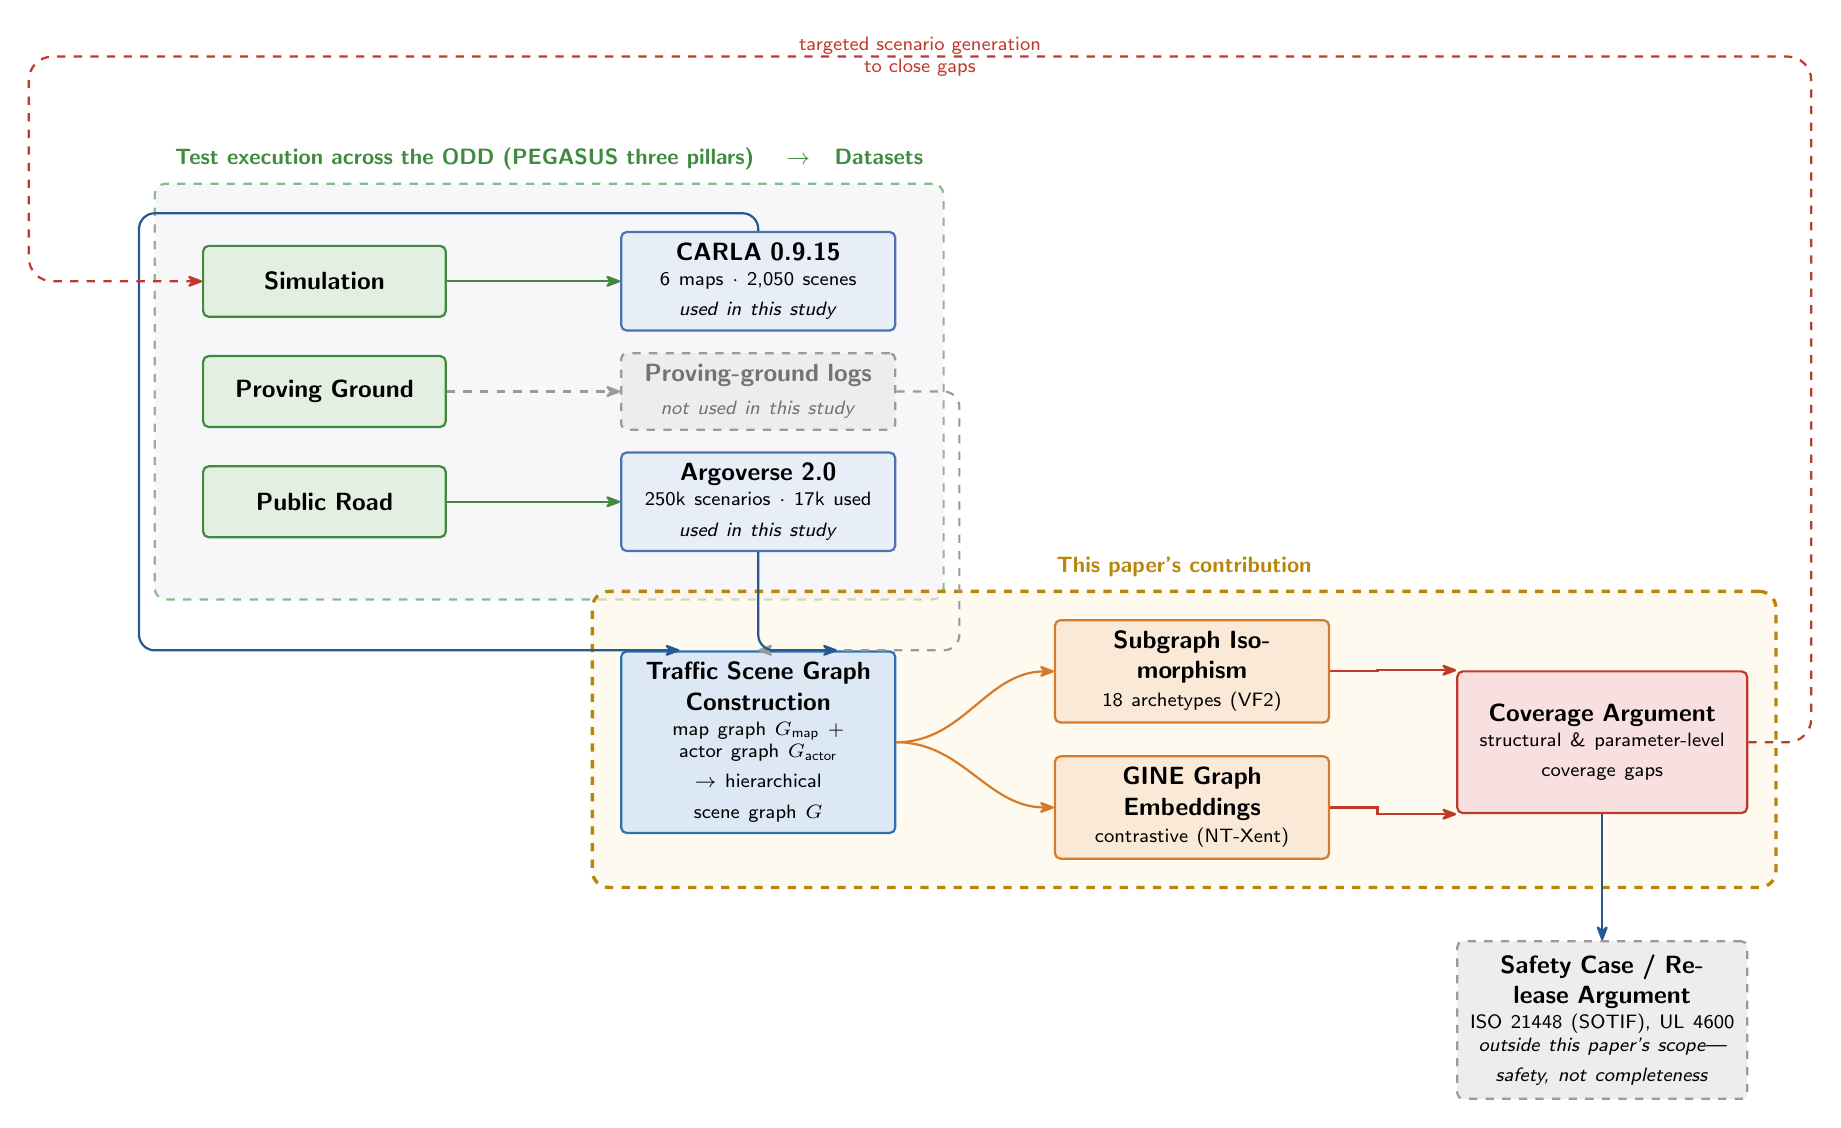
\begin{tikzpicture}[
  font=\sffamily\small,
  >={Stealth[round]},
  node distance=6mm,
  block/.style={rounded corners=2pt,draw,thick,align=center,inner sep=4pt,minimum height=9mm},
  io/.style     ={block,fill=cInput,draw=cInputB},
  conv/.style   ={block,fill=cConv,draw=cConvB},
  pool/.style   ={block,fill=cPool,draw=cPoolB},
  head/.style   ={block,fill=cHead,draw=cHeadB},
  loss/.style   ={block,fill=cLoss,draw=cLossB},
  ext/.style    ={block,fill=cMuted,draw=cMutedB,dashed},
  muted/.style  ={block,fill=cMuted,draw=cMutedB,dashed,text=black!55},
  flow/.style   ={->,thick,cConvB!80!black},
  dimlab/.style ={font=\sffamily\scriptsize\itshape,text=black!60},
  grp/.style    ={rounded corners=4pt,draw=black!35,dashed,thick,fill=cGroup,inner sep=7pt},
  grptitle/.style={font=\sffamily\bfseries\footnotesize,text=black!70},
  contrib/.style={rounded corners=6pt,draw=cContribB,dashed,very thick,fill=cContrib,fill opacity=0.55,inner sep=10pt},
]

% =====================================================================
% LAYER 1 (top): TEST EXECUTION -- THREE PILLARS -- AND DATASETS
% =====================================================================
\node[pool,text width=28mm] (sim)     at (0,1.4)  {\textbf{Simulation}};
\node[pool,text width=28mm] (proving) at (0,0)    {\textbf{Proving Ground}};
\node[pool,text width=28mm] (road)    at (0,-1.4) {\textbf{Public Road}};

\node[io,right=22mm of sim,text width=32mm] (carla)
  {\textbf{CARLA 0.9.15}\\[1pt]\scriptsize 6 maps $\cdot$ 2{,}050 scenes\\\scriptsize\textit{used in this study}};
\node[muted,right=22mm of proving,text width=32mm] (pg)
  {\textbf{Proving-ground logs}\\[1pt]\scriptsize\textit{not used in this study}};
\node[io,right=22mm of road,text width=32mm] (argo)
  {\textbf{Argoverse 2.0}\\[1pt]\scriptsize 250k scenarios $\cdot$ 17k used\\\scriptsize\textit{used in this study}};

\draw[flow,cPoolB] (sim.east) -- (carla.west);
\draw[flow,cMutedB,dashed] (proving.east) -- (pg.west);
\draw[flow,cPoolB] (road.east) -- (argo.west);

\begin{scope}[on background layer]
  \node[grp,fit=(sim)(proving)(road)(carla)(pg)(argo),draw=cPoolB!60,inner sep=6mm] (PILLARS) {};
\end{scope}
\node[grptitle,above=1pt of PILLARS.north,text=cPoolB,align=center]
  {Test execution across the ODD (PEGASUS three pillars) \quad$\rightarrow$\quad Datasets};

% =====================================================================
% LAYER 2 (middle): THIS PAPER'S CONTRIBUTION
% =====================================================================
\node[conv,text width=32mm,minimum height=22mm]
  (graph) at ($(PILLARS.south -| carla)+(0,-18mm)$)
  {\textbf{Traffic Scene Graph Construction}\\[1pt]
   \scriptsize map graph $G_{\text{map}}$ + actor graph $G_{\text{actor}}$\\
   \scriptsize $\rightarrow$ hierarchical scene graph $G$};

% CARLA, proving-ground and Argoverse are stacked in one column above
% graph; route each around the boxes below/beside it instead of through.
\coordinate (carlaBypassX) at ($(sim.west)+(-8mm,0)$);
\coordinate (carlaTopY) at ($(sim.north)+(0,4mm)$);
\draw[flow,rounded corners=2mm]
  (carla.north) -- (carla.north |- carlaTopY) -- (carlaBypassX |- carlaTopY) -- (carlaBypassX |- graph.north) -- ($(graph.north)+(-10mm,0)$);

\coordinate (pgBypassX) at ($(pg.east)+(8mm,0)$);
\draw[flow,cMutedB,dashed,rounded corners=2mm]
  (pg.east) -- (pgBypassX |- pg.east) -- (pgBypassX |- graph.north) -- (graph.north);

\draw[flow,rounded corners=2mm]
  (argo.south) -- (argo.south |- graph.north) -- ($(graph.north)+(10mm,0)$);

\node[head,right=20mm of graph,yshift=9mm,text width=32mm] (subiso)
  {\textbf{Subgraph Isomorphism}\\[-1pt]\scriptsize 18 archetypes (VF2)};
\node[head,below=4mm of subiso,text width=32mm] (gine)
  {\textbf{GINE Graph Embeddings}\\[-1pt]\scriptsize contrastive (NT-Xent)};

\draw[flow,cHeadB] (graph.east) to[out=0,in=180] (subiso.west);
\draw[flow,cHeadB] (graph.east) to[out=0,in=180] (gine.west);

\node[loss,right=16mm of subiso,yshift=-9mm,text width=34mm,minimum height=18mm] (argument)
  {\textbf{Coverage Argument}\\[1pt]\scriptsize structural \& parameter-level\\\scriptsize coverage gaps};

\draw[flow,cLossB] (subiso.east) -- ++(6mm,0) |- (argument.north west);
\draw[flow,cLossB] (gine.east)   -- ++(6mm,0) |- (argument.south west);

\begin{scope}[on background layer]
  \node[contrib,fit=(graph)(subiso)(gine)(argument)] (CONTRIB) {};
\end{scope}
\node[grptitle,above=1pt of CONTRIB.north,text=cContribB] {This paper's contribution};

% =====================================================================
% LAYER 3 (bottom, right-aligned): SAFETY CASE -- EXTERNAL / OUT OF SCOPE
% =====================================================================
\node[ext,text width=34mm,minimum height=20mm,anchor=north east]
  (safety) at ($(argument.south east)+(0,-16mm)$)
  {\textbf{Safety Case / Release Argument}\\[1pt]\scriptsize ISO~21448 (SOTIF), UL~4600\\
   \scriptsize\textit{outside this paper's scope---}\\\scriptsize\textit{safety, not completeness}};

\draw[flow] (argument.south) -- (safety.north);

% =====================================================================
% FEEDBACK LOOP (routed along the outer right/top/left margin, clear of
% all boxes, closing the loop on the left side of the Simulation box)
% =====================================================================
\coordinate (fb1) at ($(argument.east)+(8mm,0)$);
\coordinate (fbTopY) at ($(PILLARS.north)+(0,16mm)$);
\coordinate (fb2) at (fb1 |- fbTopY);
\coordinate (feedbackLeftX) at ($(sim.west)+(-22mm,0)$);
\coordinate (fb3) at (feedbackLeftX |- fb2);
\coordinate (fb4) at (feedbackLeftX |- sim.west);
\draw[->,thick,cLossB,dashed,rounded corners=3mm]
  (argument.east) -- (fb1) -- (fb2) -- (fb3) -- (fb4) -- (sim.west);
\node[font=\sffamily\scriptsize,text=cLossB,align=center] at ($(fb2)!0.5!(fb3)$)
  {targeted scenario generation\\to close gaps};

\end{tikzpicture}
\end{document}
